\documentclass[11pt,ngerman,a4paper]{article}
%Gummi|061|=)
\usepackage{amsmath}
\usepackage{a4wide}
\usepackage{url}
\usepackage{amsthm}
\usepackage{amsbsy}
\usepackage{amssymb}
\usepackage[utf8]{inputenc}
\usepackage{rotating}
\usepackage{here}
\usepackage{graphicx}
\usepackage{paralist}
\usepackage{selinput}
\usepackage[separate-uncertainty=true]{siunitx}
\usepackage{booktabs}
\sisetup{}
\SelectInputMappings{%
adieresis={ä},
germandbls={ß},
}
\title{\textbf{Versuch V504: Thermische Elektronenemission}}
\author{Martin Bieker\\
Julian Surmann\\
\\
Durchgef\"{u}hrt am 17.06.2014\\
TU Dortmund}
\date{}
\usepackage{graphicx}
\begin{document}
\renewcommand\tablename{Tabelle}
\renewcommand\figurename{Abbildung}
\maketitle
\thispagestyle{empty}
\newpage
\clearpage
\setcounter{page}{1}


\section{Einleitung}
In diesem Versuch wird die sogenannte Thermische Elektronenemission untersucht, dabei handelt es sich um die Auslösung von Elektronen aus einer Metalloberfläche mit Hilfe von thermischer Energie. Die Temperaturabhängigkeit dieses Vorganges ist von besonderem Interesse.
\section{Theorie}
Metalle besitzen eine sehr gute Leitfähigkeit, da praktisch alle auf den Kristallgitterplätzen sitzenden Atome ionisiert sind. Die daraus resultierenden freien Elektronen werden Leitungselektronen genannt. Das Potential der Gitterstruktur lässt sich als konstant betrachten. Damit lässt sich Metallplatte im Raum mit dem Potentialtopfmodell vergleichen. Die Elektronen können sich innerhalb des Metalles frei bewegen. Wenn ein Elektron den Leiter jedoch verlassen will, muss es eine Austrittsarbeit leisten, um die Potentialbarriere zu überwinden. Aus der Quantentheorie folgen zwei Bedingungen: Die Elektronen können nur diskrete Energiewerte annehmen und zu jedem Zustand mit einer Energie $E_n$ darf es nur zwei Elektronen geben, die sich im Spin unterscheiden (Pauli-Verbot). Aus letzerer folgt, dass die Elektronen selbst bei $T = \SI{0}{\kelvin}$ eine Energie besitzen müssen. In diesem Zustand bezeichnet man die maximale Energie eines Elektrons als Fermische Grenzenergie $\zeta$. Diese ist abhängig von der Elektronendichte. Die Fermi-Diracsche Verteilungsfunktion
\begin{equation}
f(E) = \frac{1}{e^{\frac{E-\zeta}{k T}}+1}
\end{equation}
gibt die Warscheinlichkeit an, dass ein möglicher Zustand mit der Energie E besetzt ist.
Abbildung \ref{funktion} zeigt den Verlauf der Fermi-Diracschen Verteilungsfunktion am Beispiel des Absoluten Nullpunktes und einer Temperatur $T >> 0$.
\newline
Die Anzahl der Elektronen pro Volumeneinheit des Phasenraumes (aufgespannt durch Impuls- und Ortskoordinaten) lässt sich mit Hilfe von
\begin{equation}
n(E) = \frac{2}{h^3}f(E)
\end{equation}
berechnen. Die Richardson-Gleichung für die Stromdichte in Abhängigkeit von der Temperatur ergibt sich zu
\begin{equation}
j_s(T) = \frac{4\pi e_0 m_0 k^2}{h^3} T^2 e^{\frac{-e_0 \phi}{k T}}.
\end{equation}
\subsection{Die Hochvakuum-Diode}
Eine Messung des Sättigungsstromes der emittierenden Metalloberfläche ist nur im Hochvakuum möglich, da die austretenden Eletronen sonst in Wechselwirkung mit den Gasmolekülen treten würden. Die Hochvakuum-Diode ist nicht nur evakuiert, in ihr lässt sich auch ein elektrisches Feld erzeugen.\newline
Die Hochvakuum-Diode besteht aus einem evakuierten Glaskörper, in dem ein Draht angebracht ist. Durch eine angelegte Spannung fließt Strom durch diesen (Wolfram-)Draht, der so auf 1000-$\SI{3000}{\kelvin}$ erhitzt wird. Zwischen der Glühkathode und einer gegenüber liegenden Anode kann mit einer weiteren angelegten Spannung das elektrische Feld erzeugt werden, um die freien Elektronen abzusaugen.
\subsection{Die Langmuir-Schottkysche Raumladungsgleichung}
\section{Auswertung}
\subsection{Bestimmung des Sättigungsstroms}
Zur Bestimmung des temperaturabhängigen Sättigungsstroms der Diode wurde der Strom in Abhängigkeit vom der Spannung zwischen Anode und Kathode gemessen. Diese Daten befinden sich in Tabelle \ref{tab_a}. In Abbildung \ref{abb_a} werden die ermittelten Kennlinien graphisch dargestellt. 
\begin{figure}[htp]
\centering
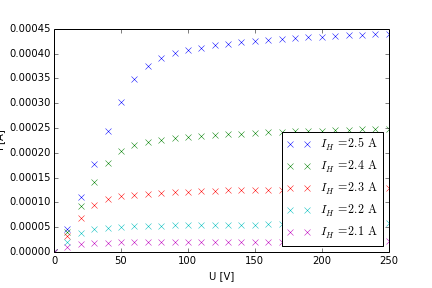
\includegraphics[scale=0.8]{plot_a.png}
\caption{Kennlinie der Hochvakuumdiode in Abhängigkeit von der Temperatur.}
\label{abb_a}
\end{figure}

\noindent
Es ist erkennbar, dass der Strom innerhalb des untersuchten Spannungsbereichs das jeweilige temperaturabhängige Sättigungsniveau erreicht. Somit entspricht der Sättigungsstrom näherungsweise dem höchsten gemessenen Wert von $I$ der jeweiligen Messreihe. Daher gilt:
\begin{itemize}
\item $I_{S1} = \SI{440}{\micro\ampere}$
\item $I_{S2} = \SI{248}{\micro\ampere}$
\item $I_{S3} = \SI{129}{\micro\ampere}$
\item $I_{S4} = \SI{58}{\micro\ampere}$
\item $I_{S5} = \SI{22}{\micro\ampere}$
\end{itemize}

\subsection{Verifizierung Langmuir-Schottkyschen Gesetztes}
In diesem Versuchsteil wird das Raumladungsgebiet der Kennlinie genauer untersucht.
Hier soll der Exponent $q$ der Strom-Spannungsbeziehung 
\[
I = k\cdot x^q
\]
bestimmt werden. Dazu sind in Abbildung \ref{plot_b} sind die Messpunkte für die maximale Heizleistung ($I_H = \SI{2.5}{\ampere}$) doppelt logarithmisch aufgetragen.

\begin{figure}[htp]
\centering
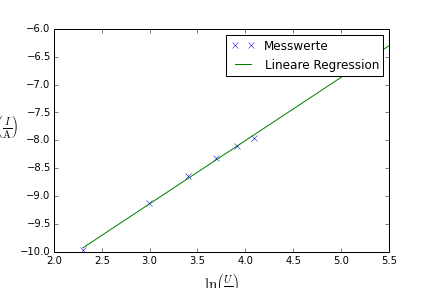
\includegraphics[scale=0.80]{plot_b.png}
\caption{Doppelt-Logarithmische Darstellung der Diodenkennline im Raumladungsgebiet mit $I_H = \SI{2.5}{\ampere}$}
\label{plot_b}
\end{figure}

\noindent
In dieser Darstellung ist der lineare Zusammenhang
\[
\ln\left(\frac{I}{\si{\ampere}}\right) = q\cdot \ln\left(\frac{U}{\si{\volt}}\right)+ \ln\left(\frac{k}{\si{\ampere\per\volt}}\right)
\]
erkennbar. Durch eine lineare Ausgleichsrechnung ergibt sich:
\begin{itemize}
\item $q = \num{1.1317+-0.0011}$
\item $\ln\left(\frac{k}{\si{\ampere\per\volt}}\right) = \num{-12.531+-0.013}$ 
\end{itemize}
Die durch diese Werte bestimmte Ausgleichsgerade ist ebenfalls in Abbildung \ref{plot_b} dargestellt.
Die Abweichung von $q$ zum Langmuir-Schottkyschen Gesetz mit 
\[
q_{theo} = \frac32
\]
beträgt:
\[
\Delta q = \frac{|q_{theo}-q|}{q_{theo}} = \SI{24.55}{\percent}\rm.
\]
\subsection{Untersuchung des Anlaufstromgebiets}
Tabelle \ref{tab_c} enthält den gemessenen Diodenstrom $I$ in Abhängigkeit von der angelegten Gegenspannung $U$. Da aber das zur Messung des Stroms verwendete Amperemeter einen nicht vernachlässigbaren Innenwiderstand
\[
R_i = \SI{1}{\mega\ohm}
\]
besitzt, muss die gemessenen Werte für die Spannung zunächst korrigiert werden. Gemäß der Kirchhoffschen Maschenregel gilt für die Spannung zwischen Anode und Kathode:
\[
U_{Korr} = U_{Messung} + I \cdot R_i
\]
Die korrigierten Werte sind in Abbildung \ref{plot_c_lin} graphisch dargestellt.
\begin{figure}[htp]
\centering
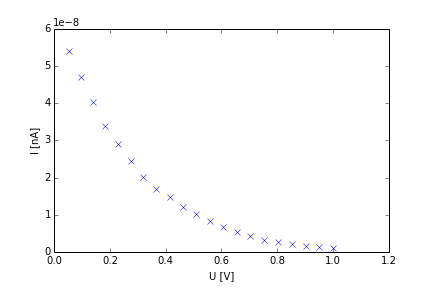
\includegraphics[scale=0.8]{plot_c_lin.png}
\caption{Strom in Abhängigkeit von der Gegenspannung im Anlaufstromgebiet der Diode.}
\label{plot_c_lin}
\end{figure}
\noindent
Es zeigt sich der erwartete exponentielle Zusammenhang
\[
I = C\cdot \exp\left(\frac{e_0 U}{k_b T}\right)\rm.
\]
Daher werden die Messwerte in Abbildung \ref{plot_c_log} halb-logarithmisch aufgetragen. 
\begin{figure}[htp]
\centering
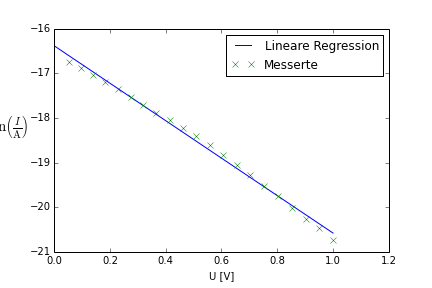
\includegraphics[scale=0.80]{plot_c_log.png}
\caption{Halb-Logarithmische Darstellung des Stroms in Abhängigkeit von der Gegenspannung.}
\label{plot_c_log}
\end{figure}
\noindent
Es ergibt sich der folgende lineare Zusammenhang:
\[
\ln{\left(\frac{I}{\si{\ampere}}\right)} = \frac{e_0}{k_b T }\cdot U + \ln(C)\rm = m \cdot U + b.
\]
Durch eine lineare Regression wird die Steigung $m$ der Geraden bestimmt. Es ergibt sich:
\[
m = \num{-4.198+-0.004} = \frac{e_0}{k_b T} \Leftrightarrow T = \SI{2764.2+-2.7
}{\kelvin}
\] 
\subsection{Bestimmung der Temperatur der Kathode}

Aus einer Leistungsbilanz kann die Temperatur der Kathode bestimmt werden. Denn es gilt:
\[
N_{el} = N_{WL} + N_{Str.}\rm.
\]
Die Elektrische Heizleistung kann aus Heizstrom und Heizspannung berechnet werden. Die Strahlungsleistung kann durch das Stefan-Boltzmannsche Gesetz
\[
N_{Str.} = A \eta\sigma T^4
\]
ausgedrückt werden. Da die Fläche der Kathode 
\[
A = \SI{0,32}{\centi\meter\squared}
\]
die Stefan-Boltzmannsche Konstante 
\[
\sigma = \SI{}{\watt\per(\centi\meter\squared\kelvin^4)}
\]
und der Absorptionsgrad
\[
\eta = \num{0,27}
\]
bekannt sind und der Energieverlust durch Wärmeleitung durch
\[
N_{WL} = \SI{1}{\watt}
\]
abgeschätzt werden kann, gilt für die Temperatur:
\[
T = \sqrt[4]{\frac{U_H I_H - \SI{1}{\watt}}{A\eta\sigma}}\rm.
\]
Die Ergebnisse dieser Berechnungen befinden sich in Tabelle \ref{tab_d}.

\subsection{Berechnung der Austrittsarbeit des Kathodenmaterials}
Aus den in den vorherigen Teilen der Auswertung bestimmten Werten für den Sättigungsstrom $I_S$ der dazugeörigen Kathodentemperatur $T$ kann mit Hilfe der Richardson-Gleichung (Formel \ref{}) die Austrittsarbeit des Kathodenmaterials bestimmt werden. Es gilt:
\[
W_A = -\log\left( \frac{I_S h^3}{e_0 m_0 k_b^2 T^2}\right)\cdot k_b T
\]
Die mit dieser Formel berechneten Werte befinden sich in Tabelle \ref{tab_e}. Es ergibt sich für den Mittelwert mit statistischen Fehler:
\[
 W_A = \SI{6.32+-0.05}{\eV}\rm.
\]
Die Kathode der in diesem Versuch verwendeten Diode besteht aus Wolfram. Der Literaturwert[2] für die Austrittsarbeit beträgt
\[
W_A \approx \SI{4,6}{\eV}
\]
Damit berechnet sich die Abweichung des experimentell bestimmten Wertes vom Literatur-wert zu
\[
\Delta W_A = \frac{|W_A-\overline{W_A}|}{W_A} = \SI{38,79}{\percent} 
\]

\section{Diskussion}

\section{Quellen}
\begin{enumerate}[{[}1{]}]
\item Entnommen der Praktikumsanleitung \textit{} der TU Dortmund. \\
Download am 01.06.14 unter:\\
 \url{http://129.217.224.2/HOMEPAGE/PHYSIKER/BACHELOR/AP/SKRIPT/V703.pdf}
\end{enumerate}

\section{Anhang}
\begin{itemize}
\item Tabellen
\item Auszug aus dem Messheft
\end{itemize}
\newpage


\begin{table}
\centering
\begin{tabular}{l|rrrrr}
\toprule
$\frac{U}{\si{\volt}} $&$\frac {I_1}{\si{\micro\ampere}}$&$\frac {I_2}{\si{\micro\ampere}}$ &$\frac {I_3}{\si{\micro\ampere}}$&$\frac {I_4}{\si{\micro\ampere}}$&$\frac {I_5}{\si{\micro\ampere}}$\\
\midrule
0 & 0 & 0 & 0 & 0 & 0\\
10 & 47 & 40 & 32 & 21 & 11\\
20 & 110 & 92 & 68 & 38 & 16\\
30 & 177 & 142 & 94 & 46 & 18\\
40 & 244 & 180 & 107 & 49 & 19\\
50 & 303 & 203 & 112 & 51 & 20\\
60 & 348 & 215 & 115 & 52 & 20\\
70 & 375 & 222 & 117 & 53 & 20\\
80 & 391 & 226 & 119 & 53 & 20\\
90 & 402 & 229 & 120 & 54 & 21\\
100 & 407 & 232 & 121 & 54 & 21\\
110 & 412 & 233 & 122 & 54 & 21\\
120 & 417 & 235 & 123 & 55 & 21\\
130 & 420 & 237 & 124 & 55 & 21\\
140 & 423 & 238 & 124 & 55 & 21\\
150 & 425 & 240 & 125 & 55 & 21\\
160 & 427 & 241 & 125 & 56 & 21\\
170 & 429 & 242 & 126 & 56 & 21\\
180 & 431 & 243 & 126 & 56 & 22\\
190 & 433 & 244 & 127 & 56 & 22\\
200 & 434 & 244 & 127 & 57 & 22\\
210 & 436 & 245 & 128 & 57 & 22\\
220 & 437 & 246 & 128 & 57 & 22\\
230 & 438 & 247 & 128 & 57 & 22\\
240 & 439 & 247 & 129 & 57 & 22\\
250 & 440 & 248 & 129 & 58 & 22\\
\bottomrule
\end{tabular}

\caption{Messwerte zur Bestimmung der Kennlinie der Diode bei verschiedenen Temperaturen.}
\label{tab_a}
\end{table}


\begin{table}
\centering
\begin{tabular}{Srr}
\toprule
$\frac{U}{\si{\volt}}$ & $\frac{U_{korr}}{\si{\volt}}$&$\frac {I_1}{\si{\nano\ampere}}$\\
\midrule
0 & 0.054 & 54.00\\
0.05 & 0.097 & 47.00\\
0.10 & 0.140 & 40.25\\
0.15 & 0.184 & 34.00\\
0.20 & 0.229& 29.00\\
0.25 & 0.275& 24.50\\
0.30 & 0.320& 20.25\\
0.35 & 0.367& 17.00\\
0.40 & 0.415 & 14.75\\
0.45 & 0.462 & 12.20\\
0.50 & 0.510 & 10.20\\
0.55 & 0.558 & 8.25\\
0.60 & 0.607 & 6.70\\
0.65 & 0.655 & 5.35\\
0.70 & 0.704 & 4.25\\
0.75 & 0.753 & 3.35\\
0.80 & 0.803 & 2.65\\
0.85 & 0.852 & 2.05\\
0.90 & 0.902 & 1.60\\
0.95 & 0.951 & 1.30\\
1.00 & 1.001 & 1.00\\
\bottomrule
\end{tabular}

\caption{Strom in Abhängigkeit von der (korrigierten) Gegenspannung im Anlaufstromgebiet.}
\label{tab_c}
\end{table}


\begin{table}
\centering
\begin{tabular}{ccc}
\toprule
$\frac{I_H}{\si{\ampere}}$& $\frac{U_H}{\si{\volt}}$ &{ $\frac{T}{\si{\kelvin}}$}\\
\midrule
2.50 & 4.90 & 2166\\
2.40 & 4.60 & 2106\\
2.30 & 4.30 & 2043\\
2.20 & 4.05 & 1984\\
2.10 & 3.80 & 1923\\
\bottomrule
\end{tabular}
\caption{Messwerte zur Berechnung der Kathodentemperatur und die Ergebnisse.}
\label{tab_d}
\end{table}


\begin{table}
\centering
\begin{tabular}{ccc}
\toprule
$\frac{I_S}{\si{\micro\ampere}}$&$\frac{T}{\si{\kelvin}}$ &$\frac{W_A}{\si{\eV}}$\\
\midrule
440 & 2166 & 6.45\\
248 & 2106 & 6.37\\
129 & 2043 & 6.28\\
58 & 1984 & 6.22\\
22 & 1923 & 6.18\\
\bottomrule
\end{tabular}
\caption{Messwerte zur Berechnung der Austrittsarbeit und die Ergebnisse.}
\label{tab_e}

\end{table}

\end{document}
